\documentclass{article}
\usepackage[utf8]{inputenc}
 \usepackage{enumerate}
 \usepackage[T1]{fontenc}
\usepackage{cite}
%\usepackage{caption}
%\usepackage{subcaption}
\usepackage{mathtools}
\usepackage{stackengine}
\def\delequal{\mathrel{\ensurestackMath{\stackon[1pt]{=}{\scriptstyle\Delta}}}}
\usepackage{amsmath,amssymb,amsfonts}
\usepackage{amsmath,epsfig,cite,amsfonts,amssymb,psfrag,subfigure}
\usepackage{graphicx}
\usepackage{blindtext}
\usepackage{textcomp}
\usepackage{xcolor}
\usepackage{algorithm}
\usepackage[noend]{algpseudocode}
\usepackage{amsthm}
\def\BibTeX{{\rm B\kern-.05em{\sc i\kern-.025em b}\kern-.08em
    T\kern-.1667em\lower.7ex\hbox{E}\kern-.125emX}}
\allowdisplaybreaks
\newtheorem{remark}{Remark}
\newtheorem{theorem}{Theorem}
\newtheorem{lemma}{Lemma}
\newtheorem{proposition}{Proposition}
\newtheorem{corollary}{Corollary}
\newcommand{\diag}{\mathop{\mathrm{diag}}}
\DeclareMathOperator{\E}{\mathbb{E}}
\usepackage[margin=0.7in]{geometry}
\usepackage[export]{adjustbox}

\title{Reporte de inventario de eviencias}
\author{Natalia Galeano Valerio}
\date{Octubre 2019}

\begin{document}


\baselineskip 12pt

\vspace*{30mm}

\begin{center}

\textbf{\Large Research Plan} \\
\vspace{10mm}
\textbf{Department of Electrical and Computer Engineering}\\
\vspace{20mm}
{\large University of Oulu}\\
\vspace{20mm}
\end{center}
\vspace{10mm}
{\scriptsize Provisional title:}\\
Dynamic Resource Allocation in O-RAN Architecture using Network Slicing\\

\vspace{20mm}

{\scriptsize Candidate name}\\
Mojdeh Karbalaee Motalleb \\
\vspace{3mm}



{\scriptsize Supervisor name:}\\
Dr. Onel Lopez\\
\vspace{3mm}


\pagebreak
\begin{abstract}
Open radio access network (O-RAN) is the next generation of RAN systems introduced by the O-RAN Alliance to increase the flexibility and the openness of the network systems and simultaneously decrease CAPEX and OPEX of mobile operators. The O-RAN system combines and takes advantage of Cloud RAN (C-RAN) and the Virtual RAN (VRAN).
O-RAN separates RAN into three
different units, namely Radio Unit (O-RU), Distributed Unit
(O-DU), and Central Unit (O-CU).
In this research, we study
the problem of baseband resource allocation and virtual
network function (VNF) activation in O-RAN architecture
based on their service priority for different types of 5G services
including enhanced mobile broadband (eMBB), ultra-reliable
low latency communications (uRLLC) and massive Machine
Type Communications (mMTC) services using intelligent RAN slicing. 
Network slicing is a promising solution for supporting such heterogeneous and challenging services.
Deploying network slicing, the isolation of different types of services in O-DU, O-CU, and user plane function (UPF) is performed. The limited
fronthaul capacity, the restriction of end-to-end delay and the reliability of the services are
considered at the same time.
  
The optimization of baseband
resources includes O-RU assignment, the assignment of physical resource block
(PRB), and power allocation. The main problem is a mixed-integer non-linear programming problem that is tremendously difficult. Since the problem has a two-time scale, it can be broken into two layers. On the large-time scale, the problem of obtaining the optimal number of VNF, the placement of VNFs, and the assignment of PRB to the slices are considered. 
On the small-time scale, there is the problem of obtaining the optimal power of UEs, and the PRB and o-RU assignment.
To solve the problem, we propose deep reinforcement learning, the deep deterministic policy gradient (DDPG) method, and convex optimization.
\end{abstract}
\section{Introduction} 
O-RAN, as the integration and expansion of C-RAN and xRAN, or C-RAN and the vRAN is expected to be a key technology in 5G networks to enhance the RAN performance extensively. 
The core idea of C-RAN is to divide the radio remote head (RRU) from the baseband unit (BBU). Also, several BBUs are placed together to create the BBU-pool, providing unified baseband signal processing with powerful computing capabilities. On the other hand, xRAN technology has three fundamental features. The control plane is decoupled from the user plane. Besides, a modular eNB software stack is built to operate on common-off-the-shelf (COTS) hardware. Moreover, open north-bound and south-bound interfaces are introduced.
O-RAN separate RAN into three different units, namely Radio Unit (O-RU), Distributed Unit (O-DU), and Central Unit (O-CU). O-RU is a logical node that contains RF and lowers PHY. Moreover, the O-DU expresses another logical node that includes higher PHY, MAC, and RLC. In addition, the O-CU depicts the logical node contains two parts, which are the O-CU user plane (O-CU-UP) and O-CU control plane (O-CU-CP). O-CU-UP hosts PDCP-UP and SDAP, and O-CU-CP hosts PDCP-CP and RRC. O-DU and O-CU are connected via an open and well-defined interface F1.
Moreover, O-DU is connected to a radio unit (O-RU) with an open fronthaul interface.
The architecture of O-RAN contains other principal logical nodes called Orchestration and Automation,
RAN Intelligent Controller (RIC)- Near Real-Time and O-Cloud. 
One of the necessities of the new generation of wireless networks is its intelligence.
Based on the requirement of an intelligent wireless network, O-RAN offers machine learning techniques. The two logical nodes RIC-Non Real-Time (which is placed in Orchestration and Automation node) and RIC- Near Real Time, implement the algorithms for network intelligence 
\cite{gavrilovska2020cloud,niknam2020intelligent,kazemifard2021minimum,both2021system,ORANArch,ORANML,lin2021toward}.
\begin{figure*}
  \centering 
    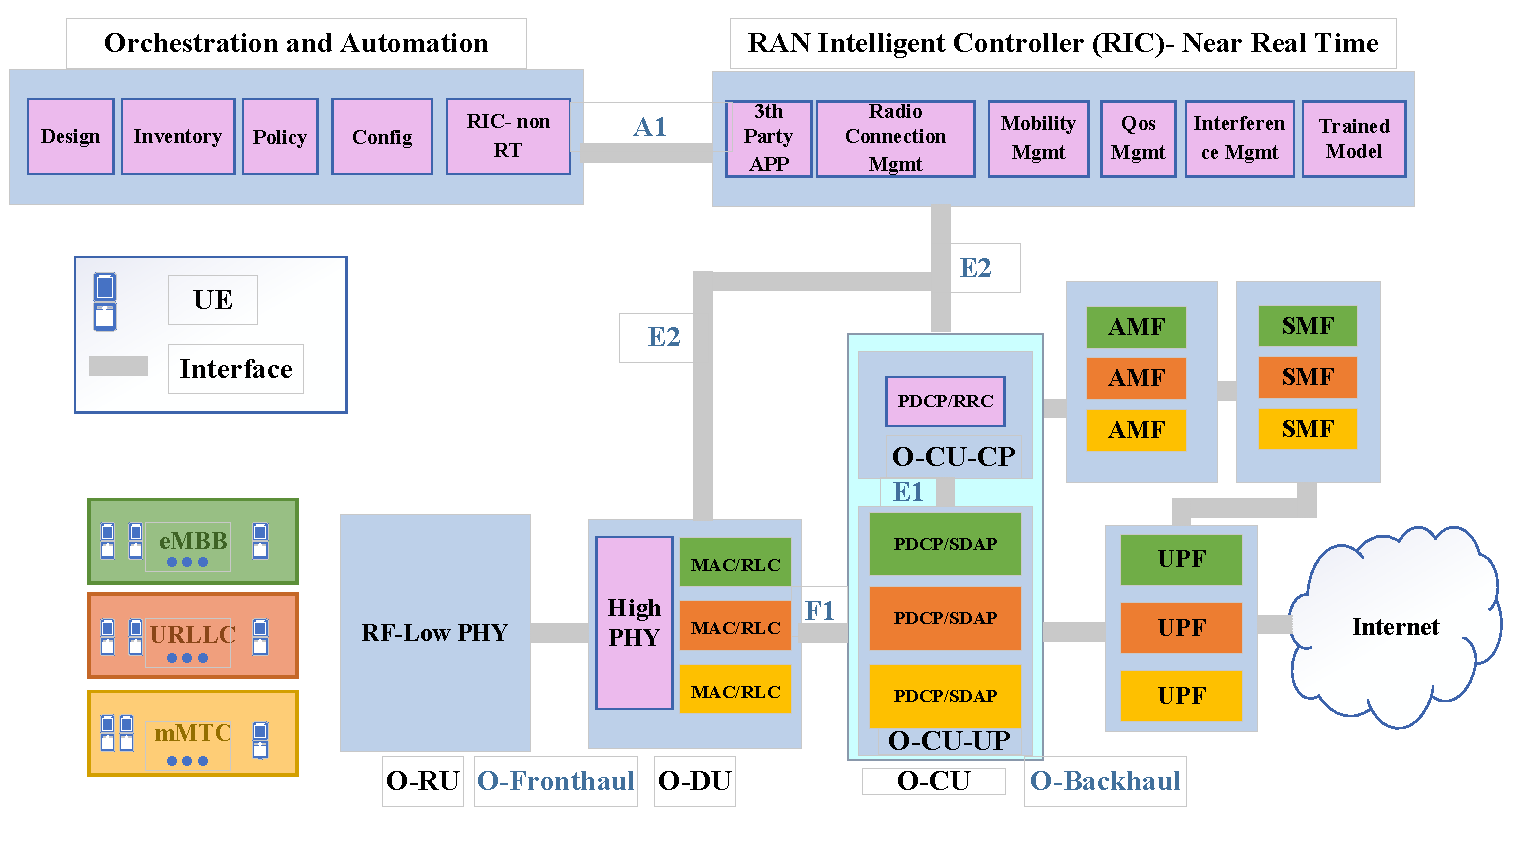
\includegraphics[scale = 0.6]{finalDraw.pdf}
    %\includegraphics[max height=30cm,max width=9.5cm]{Drawing15.eps}
    %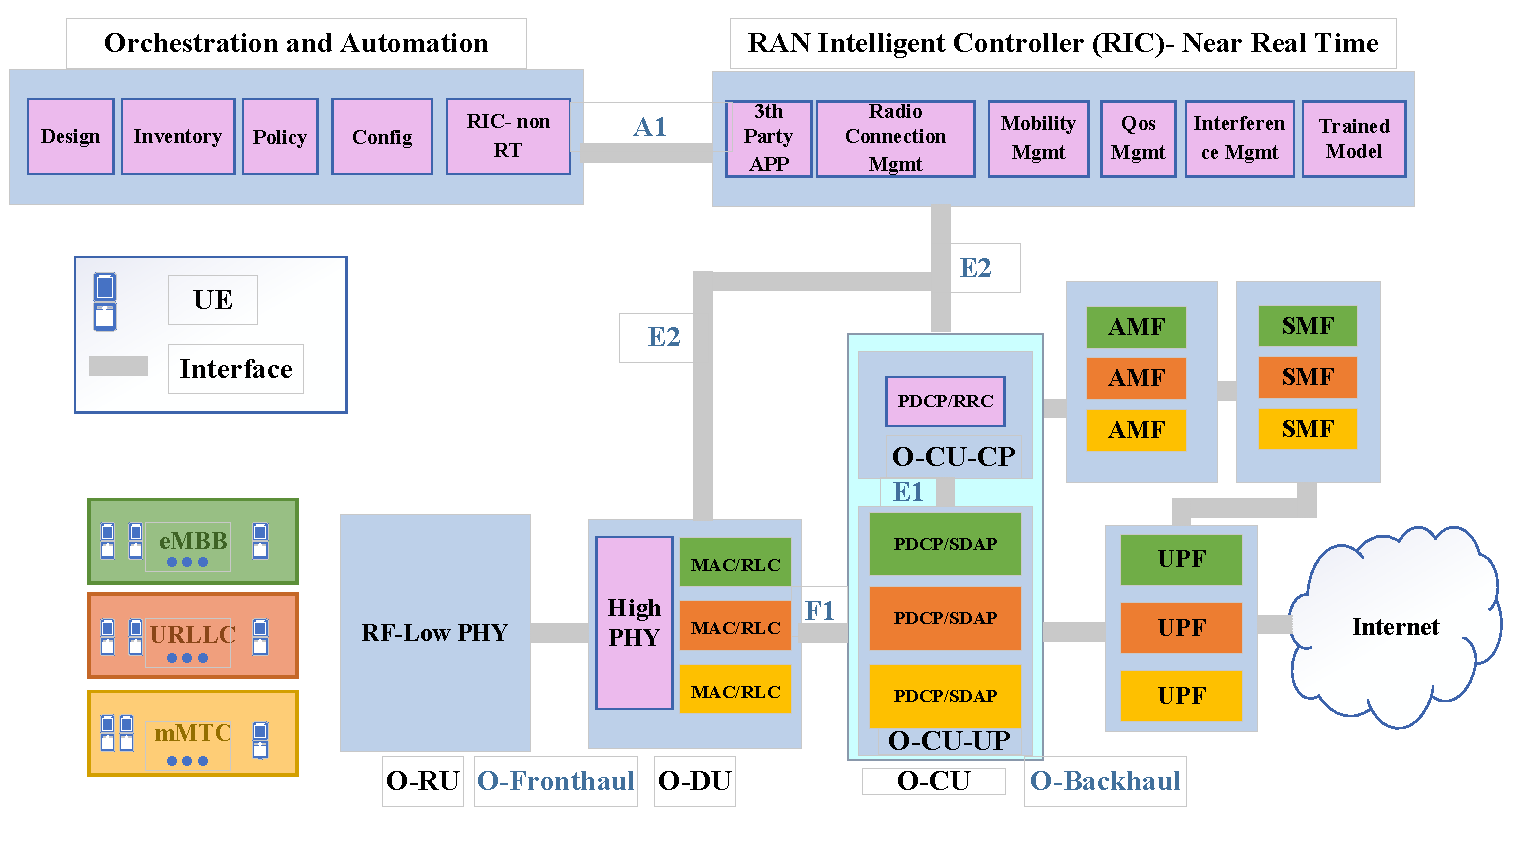
\includegraphics[width=\textwidth]{finalDraw.pdf}
  \caption{Network sliced ORAN system}
  \label{fig:c11}
\end{figure*}


One of the goals of the next generation of mobile systems is to strictly meet the stringent QoS demands of the different services introduced in 5G , i.e., eMBB, URLLC, and mMTC. Network slicing is a promising solution to obtain the QoS for each type of service. Network slicing contains RAN slicing, core slicing, and both of them together. Efficient slicing of RAN is still challenging due to time-varying network circumstances.
%Network slicing will propose significant complexity into the performance of systems that causes conventional mathematical model-based procedures to network operation no longer adequate. 
Network slicing creates considerable complexity in system performance and makes the conventional mathematical methods insufficient to model the network.
Therefore, it motivates researchers to realize network slicing using machine learning strategies such as deep learning and deep reinforcement learning. So, the network can reach the best control policy according to its experience in the past time slots.
As mentioned above, network slicing, which contains RAN slicing, core slicing, and the whole, is considered a hot topic for vendors. In addition, the O-RAN system seems to be the next RAN architecture. So, this motivated researchers to study the dynamic RAN slicing in O-RAN architecture to achieve the desired QoS for each service type.
In addition, according to the high complexity of RAN slicing and incapability of the traditional model-based methods, dynamic machine learning becomes the best solution for these problems.
 Generally, there are two kinds of deep reinforcement learning methods for solving dynamic problems. The first class is value-based such as Deep-Q-Network, and the second class is policy-based problems such as DDPG. The first class can only solve the discrete action space problems, which are integer programming. The second class can solve by searching the optimal policy, which is the actor-critic method. Here, we use the second method to solve our problems.
 


\section{Motivation and contributions}
In this project, we want to solve the problem of dynamic network slicing in the O-RAN system. The system has a two-time scale and should be solved in two layers. On a large time scale, the problem of obtaining an optimal number of VNFs and the VNF placement is performed. Also, the assignment of RB to the slices is obtained. There are three types of services that requires three types of slices: URLLC, which requires low latency; eMBB, which needs high data rate; and mMTC, short packet and low power devices.
The conventional models cannot perform well in the system because of the different QoS for each service type, and the complexity of dynamic RAN slicing. So we must switch to machine learning and dynamic methods and find the most suitable approach.  
A dynamic strategy of resource allocation is required to solve this problem to achieve the specific QoS for each type of service in the O-RAN architecture.
In this project, we want to have an intelligent resource allocation in the O-RAN architecture for the different scenarios of services. 
Also, another goal of this project is to apply transfer learning to the system and enhance the performance and the convergence of the methods. 
\section{Research Method and data set}
In this research, we want to use the machine learning methods such as deep reinforcement learning and deep learning to train the O-RAN system and have an intelligent system. The multi-agent deep reinforcement learning contains DDPG, the deep deterministic policy gradient algorithm (actor-critic algorithm), correlated q-learning, and the priority proportional fairness algorithm. 
The deep learning algorithms contain LSTM and recurrent neural networks. Also, transfer learning is an exciting way to enhance the performance and convergence of the system.


\bibliographystyle{IEEEtran} 
\bibliography{ref}
%\begin{thebibliography}{9}
%\bibitem{Hunt}
%Sally Hunt, ``Making Competition Work in Electricity,'' John Wiley , pp.23-30, Fev, 2002.



%\end{thebibliography}
\vspace{20mm}


\end{document}
